% A beamer slide deck for the compile corpus: a theme, overlays, columns, a block, maths and
% a TikZ drawing. All content is made up.
\documentclass{beamer}
\usetheme{Madrid}
\usecolortheme{beaver}
\usepackage{tikz}

\title{Example Graphs in Practice}
\author{Alex Example}
\institute{Example University}
\date{January 2026}

\begin{document}

\begin{frame}
  \titlepage
\end{frame}

\begin{frame}{Outline}
  \tableofcontents
\end{frame}

\section{Motivation}
\begin{frame}{Why example graphs?}
  \begin{itemize}
    \item<1-> They are small.
    \item<2-> They are made up.
    \item<3-> They compile quickly.
  \end{itemize}
\end{frame}

\section{Method}
\begin{frame}{Method}
  \begin{columns}
    \column{0.5\textwidth}
    \begin{block}{Degree sum}
      $\sum_{v} \deg(v) = 2|E|$
    \end{block}
    \column{0.5\textwidth}
    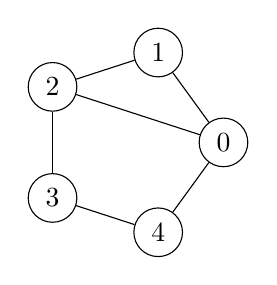
\begin{tikzpicture}
      \foreach \i in {0,...,4} \node[circle, draw] (n\i) at (72*\i:1.2) {\i};
      \foreach \i/\j in {0/1,1/2,2/3,3/4,4/0,0/2} \draw (n\i) -- (n\j);
    \end{tikzpicture}
  \end{columns}
\end{frame}

\end{document}
